% !TEX TS-program = pdflatex
% !TEX root = ../LightMicroRep.tex

%************************************************
\chapter{Fluorescence Correlation Spectroscopy}
\label{chp:FCS}
%************************************************

%----------------------------------------------------------------------------------------
%	INTRODUCTION
%----------------------------------------------------------------------------------------

\section{Introduction}
\paragraph{Aim} To distinguish cell morphologies during cell cycle through the detection of ribosomes. 
\\

Fluorescence Correlation Spectroscopy (FCS) is based on the detection of fluorescence signal from a very small volume.
It is a technique that allows one to measure concentrations and diffusion coefficients of fluorescently labelled molecules.
In this experiment, confocal microscopy (LSM) is coupled with FCS to estimate calibration parameters and convert fluorescence intensities to the concentration (of the corresponding protein) in living cells ~\cite{Politi2018}.

%----------------------------------------------------------------------------------------
%	METHODS
%----------------------------------------------------------------------------------------
\section{Methods}
Data acquisition was performed as the following:
\begin{itemize}
\item Calibration of the observation volume using AlexaFluor488 (as EGFP analog - Enhanced GFP), in FCS acquisition mode, to determine the size of the observation volume (\textit{in vitro}). 
\item Calibration of the image intensities (LSM imaging) against concentration (FCS) using monomeric EGFP expressed in yeast (\textit{in vivo}).
\item Determination of fluorescence probability through FCS of dimeric EGFP expressed in yeast (\textit{in vivo}).
\item Z-stack acquisition of protein of interest.
\end{itemize}

%----------------------------------------------------------------------------------------
%	RESULTS AND DISCUSSION
%----------------------------------------------------------------------------------------
\section{Results and Discussion}

%----------------------------------------------------------------------------------------
\subsection{Rpl3}
Proteins in yeast in this experiment are genetically expressing GFP. 
The protein is Rpl3, a Ribosomal 60S subunit protein L3, it is homologous to mammalian and bacterial ribosomal protein L3~\cite{YeaGenRpl3}. 
The measurement of the fluorescence intensity of GFP of a yeast cell is proportional to the number of ribosomes contained within it.

%----------------------------------------------------------------------------------------
\subsection{FCS}
The detectors in a modern LSM sytem are able to show a linear dependency of fluorophore concentrations and its intensities within several orders of magnitude~\cite{Politi2018}. 
In order to be able to quantify and convert the relative fluorescent intensities to physical quantities (i.e. the amount of fluorescently labelled proteins) a calibration of the dependency has to first be established. 
To this aim, FCS can be used.

%-------------
\paragraph{Observation Volume} 
\begin{figure}[h!]
\centering
\subfloat[$\tau_{D}$\label{taud}]{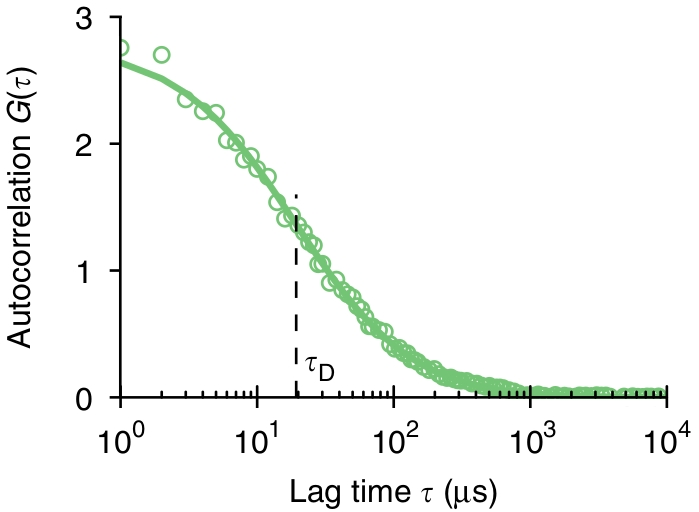
\includegraphics[width=0.25\columnwidth]{Exp_9_FCS/Figures/ACF}}\hfil
\subfloat[ACF from FCS\label{bac}]{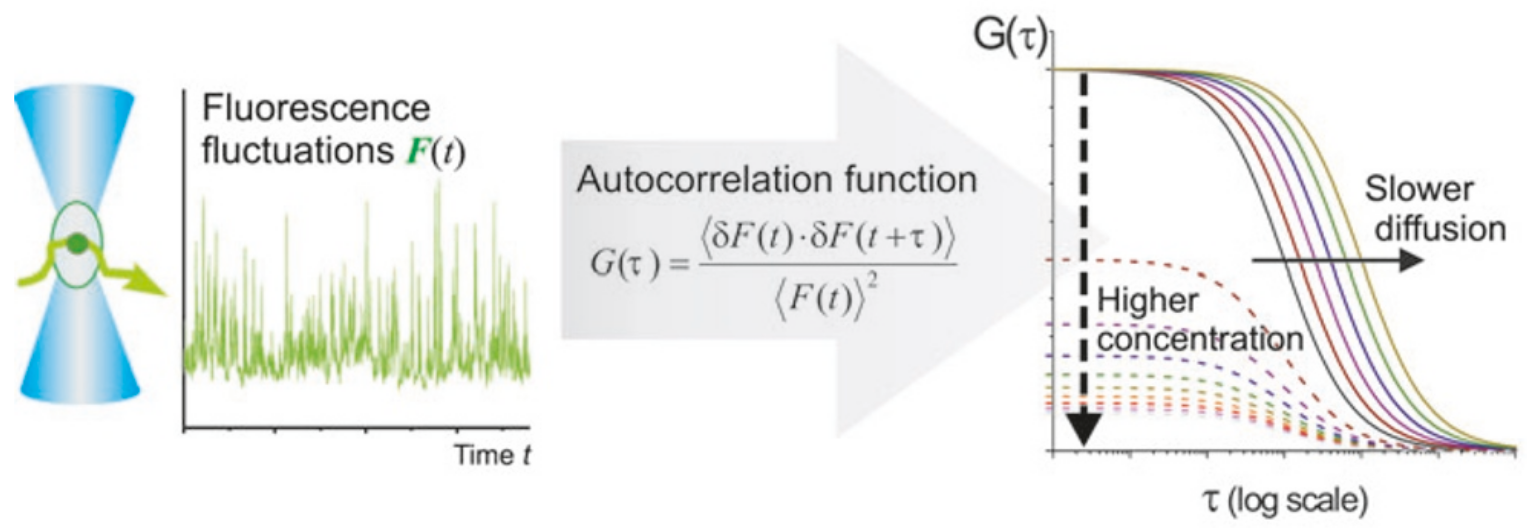
\includegraphics[width=0.55\columnwidth]{Exp_9_FCS/Figures/bac}}
\caption{\textbf{A}: Obtaining $\tau_{D}$ from ACF (taken from Politi et al~\cite{Politi2018}). \textbf{B}: Obtaining the ACF from FCS measurement (taken from Bacia et al~\cite{Bacia2006}).}
\label{fig:acf-fcs}
\end{figure}

In FCS fluorescence intensity is measured at a certain location of a sample. 
The intensity in that observation volume fluctuates with time because there is a flux of fluorescent molecules traversing the observation volume. 
The size of the observation volume is given by 
\begin{align} 
V_{\text{eff}} = \pi^{\frac{3}{2}}\,w_{0}^{2}\,z_{0}
\label{eqn:veff}
\end{align}

with $w_{0} = \sqrt{2\,(D_{dye}\,\tau_{D})}$, $z_{0} = \kappa\,w_{0}$, and $\kappa = \frac{2.33\,n}{NA}$, where $w_{0}$ and $z_{0}$ describes the dimension of the observation volume, $n$ is the refractive index, $NA$ is the numerical aperture, $D_{dye}$ is the diffusion coefficient, and $\tau_{D}$ is the average diffusion time. 
The latter is obtained by fitting the auto correlation function (ACF) to a physical model of diffusion (Fig~\ref{taud}) while the other quantities are already known either as experimental parameters ($n$ and $NA$) or as an already established value as in the case of $D_{dye}$ of EGFP.

The ACF is a correlation of a fluorescence signal with a delayed copy of itself as a function of delay. 
It is the result of the FCS measurement as illustrated in Fig.~\ref{bac}. 

%-------------
\paragraph{Fluorescence Probability}
Fluorescence measurements assumes that the amount of fluoresence being detected is proportional to the number of fluorescent molecules present. 
However fluorescent molecules can undergo many different processes that induces non-fluorescent states~\cite{Dunsing2018}. 
This introduces a challenge in interpreting the outcome of such fluorescence measurements where possibly not all molecules emit a fluorescence signal.  

A simple quantity, fluorescence probability, depicts the proportion of molecules that emit fluorescence and it is given by 
\begin{align}
p_{f}= \frac{B_{\text{dimer}}}{B_{\text{monomer}}}-1
\label{eqn:pf}
\end{align}

The fluorescence probability reflects to which degree that a fluorescent species are not fluorescently active, i.e. do not emit a signal at all. 
This is obtained through the calculation of a quantity called the brightness ($B$) of a monomeric and dimeric fluorescent species.

The brightness is given by 
\begin{align} 
B = \frac{I}{N}
\end{align} 
where $I$ is the fluorescence intensity and $N$ the number of fluorescent molecules. This relates to the y-intercept of the ACF fit (see Fig.~\ref{fig:poliacf}), or the ACF at time = 0 ($G(\tau)$ at $\tau$ = 0).  

\begin{figure}[h!]
	\centering
	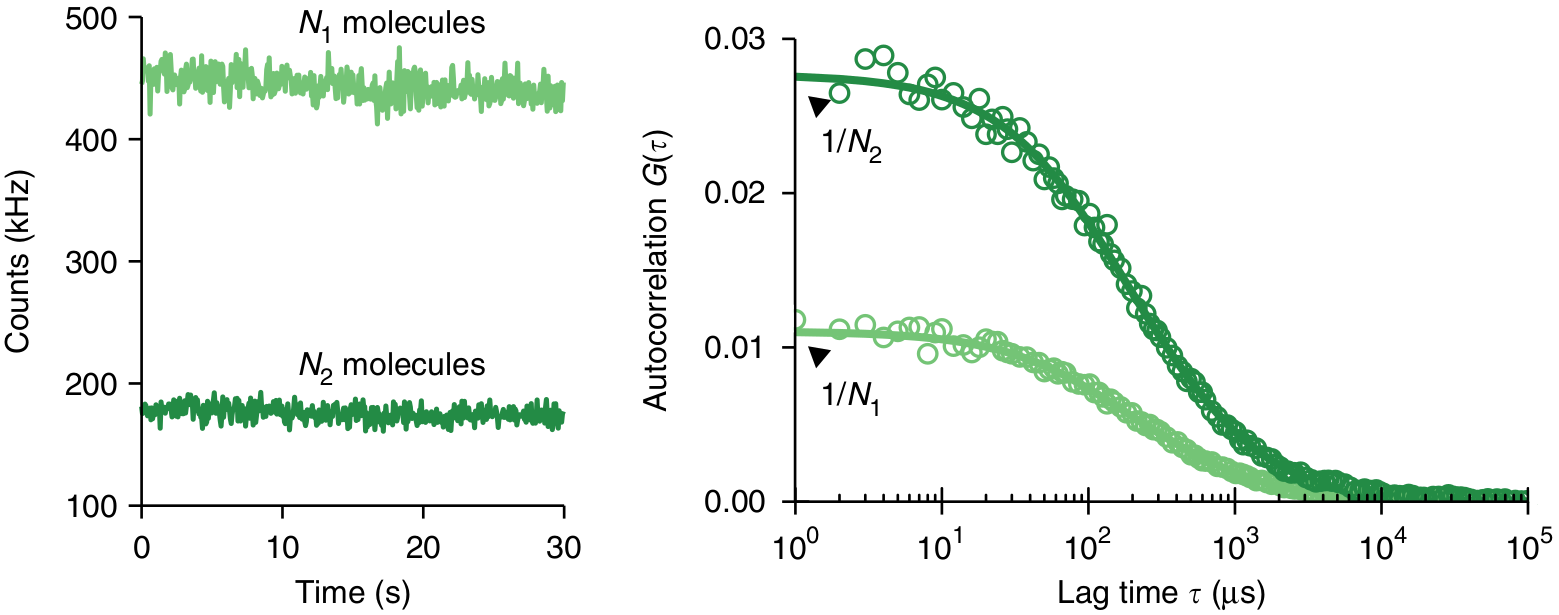
\includegraphics[width=.6\columnwidth]{Exp_9_FCS/Figures/npol}
	\caption{Relationship between $N$ and ACF fit (taken from Politi et al~\cite{Politi2018})}
	\label{fig:poliacf}
\end{figure}

%-------------
\paragraph{Corrections}
Due to the fact that fluorescent species are susceptible to bleachings during fluorescent measurements, correction of the obtained relating to this has to be performed. 
The correction is done through the ratio of the initial fluorescence intensity ($I_{0}$) and the fluorescence intensity of the measurement itself ($I$) as given by

\begin{align} 
N_{\text{corr}}=\frac{I_{0}}{I}\,N~\text{.}
\end{align} 

Also necessary to be performed alongside this is the usual background corrections. 

%-------------
\paragraph{Concentration}
Taking those factors above into account, then the concentration of the fluorescent molecules can be calculated as follows:
\begin{align} 
C=\frac{N_{\text{corr}}}{N_{A}\,V_{\text{eff}}} 
\end{align} 
where $N_{A}$ is Avogadro's constant.

%----------------------------------------------------------------------------------------
\subsection{LSM}

After establishing the necessary parameters from FCS, imaging of the protein of interest (POI) in yeast was done by by acquiring a z-stack through LSM. 
The alignment of pixel positions of the observation volume in the FCS measurements and the LSM image acquisitions were done automatically by the employed MATLAB software. 

Since in LSM the images are acquired in photon counting mode, quantities such as the brightness (or correspondingly, the intensity as well) of FCS acquisitions have to be transformed to $kHz$ with the corresponding measurement dwell time (in FCS).
\begin{align} 
B\,(\text{kHz}) = \frac{\left\langle B\right\rangle }{(\text{dwell time})_{\text{FCS}}}
\end{align}

%-------------
\paragraph{Calibration} 
The obtained concentration of the fluorescent molecules (or the POI) from FCS measurement can be calibrated with the fluorescence intensity obtained through LSM acquisition to yield a plot as exampled in Fig.~\ref{fig:monogfp}.  

%-------------
\paragraph{Concentration}
With the slope obtained by the calibration, the concentration of the POI can be calculated using the fluorescence intensity of a voxel by
\begin{align} 
[C] = \frac{I_{\text{voxel}}}{\text{slope}}
\end{align}

where the intensity of a voxel in the frequency form is
\begin{align} 
I_{\text{voxel}} = \frac{\dfrac{\sum_{j=1}^{} I}{N_{\text{voxel}}}}{(\text{dwell time})_{\text{LSM}}} 
\end{align}

with the measurement dwell time now is from the LSM acquisition. The number of voxel is the total area of each layer in a z-stack divided by the size/area of a pixel such as
\begin{align} 
N_{\text{voxel}} = \frac{\text{Area}}{\text{Pixel Area}}
\end{align}

%-------------
\paragraph{Amount of proteins}
The Rpl3 protein is in the ribosomes of yeasts and the amount of which can now be calculated according to
\begin{align} 
N_{\text{ribosome}} = [C] \cdot \text{pixel size} \cdot z_{\text{step}} \cdot N_{A} \cdot N_{\text{voxel}}
\end{align}

And finally, correcting the amount of ribosome to the fluorescence probability would then yield
\begin{align} 
N_{\text{ribosome}} = \frac{N_{\text{ribosome}}}{p_f}
\end{align}

\begin{center}
\par\noindent\rule{0.8\textwidth}{0.4pt}
\end{center}

A widefield acquisitions was performed alongside the LSM acquisitions to aid the determination of the cell cycle phase (G1/S/G2/mitosis) of the yeast cells (Mother-Bud cells). This determination was done manually as illustrated in Fig.~\ref{fig:wideyeast}. 

\begin{figure}[!h]
\centering
\captionsetup[subfigure]{position=top}
\subfloat[Yeast cell morphology\label{A}]{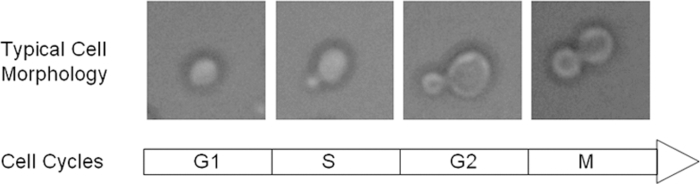
\includegraphics[width=0.6\columnwidth]{Exp_9_FCS/Figures/yeastbud}}\\\vspace{-0.7em}
\captionsetup[subfigure]{position=bottom}
\subfloat[\label{B}]{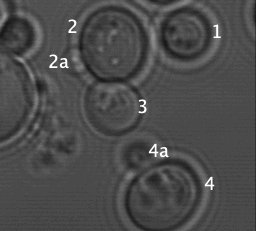
\includegraphics[width=0.25\columnwidth]{Exp_9_FCS/Figures/FCS-Image02_cr}}\hspace{0.1mm}
\subfloat[\label{C}]{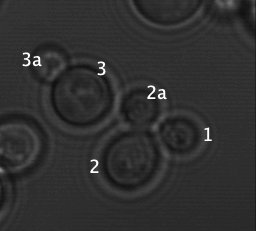
\includegraphics[width=0.25\columnwidth]{Exp_9_FCS/Figures/FCS-Image03_cr}}\\
\caption{\textbf{A}: Illustration of yeast cell morphology through cell cycle progression~\cite{Yu2011}. 
\textbf{B} and \textbf{C} are examples of widefield acquisition of yeast cells in the experiment showing the identification and numbering of mother and bud cells in different cell cycle.}
\label{fig:wideyeast}
\end{figure}

Providing that the experimental (pixel) dwell time in LSM is 12.6 $\mu$s, dwell time in FCS is 1.53 $\mu$s, pixel size is 72 nm (pixel area = 72$^{2}$ nm$^{2}$), and the z-step is 460 nm, calculations and calibrations can be done according to the above mentioned explanations.

Assuming a gaussian shaped illuminated volume, the confocal/observation volume in this experiment is 0.672 $\mu$m$^{3}$ as obtained by Eq.~\ref{eqn:veff} ($\kappa$ = 7.1) from the FCS measurement of different concentrations of monomeric AlexaFluor488 (henceforth addressed as EGFP) in solutions (\textit{in vitro}). 
The result of this measurement is then compared to the calibration of FCS measurement of monomeric EGFP expressed in yeast cells (\textit{in vivo}) to its fluorescence intensity from LSM, shown in Fig.~\ref{fig:monogfp}.  

%\begin{figure}[!h]
%\centering
%\subfloat[Monomeric EGFP in solution\label{EGFPsol}]{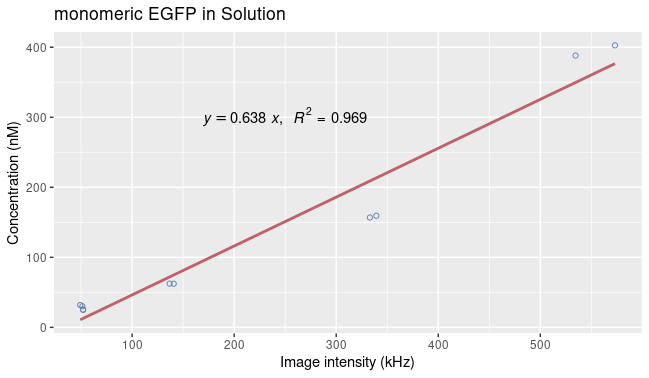
\includegraphics[width=0.5\columnwidth]{Exp_9_FCS/Figures/EGFPsol}}\hfil
%\subfloat[Monomeric EGFP-yeast\label{EGFP1}]{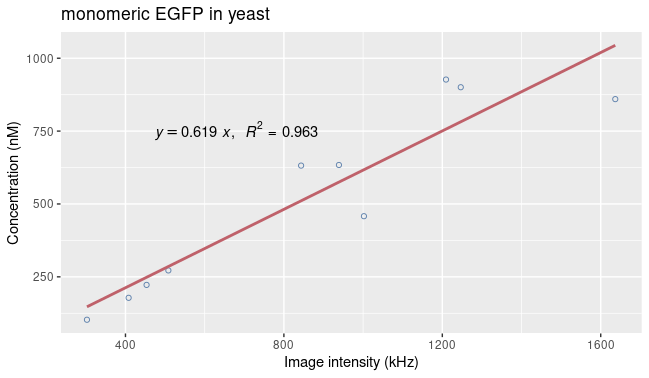
\includegraphics[width=0.5\columnwidth]{Exp_9_FCS/Figures/EGFP1}}
%\caption{Plots of concentrations against the intensity of \textbf{A}: monomeric EGFP (AlexaFluor488) in solution and \textbf{B}: yeast expressing monomeric EGFP. The concentration for \textbf{A} is obtained from calculation of FCS measurements while in \textbf{B} from LSM. 
%Both linear fits are set at 0 intercept.}
%\label{fig:monogfp}
%\end{figure}

\begin{figure}[!h]
\centering
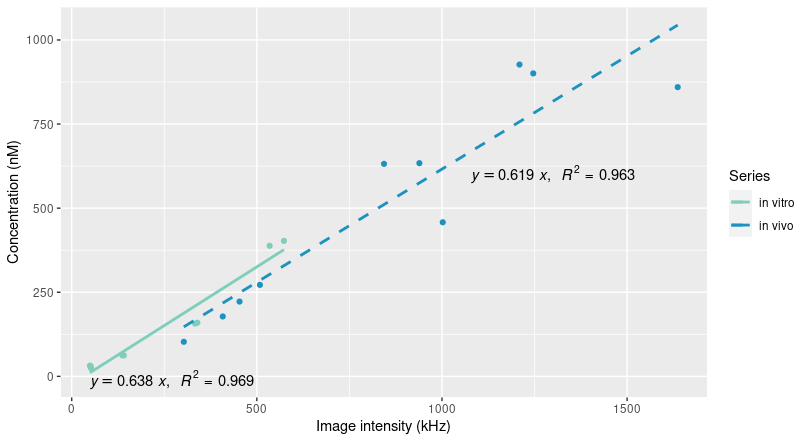
\includegraphics[width=0.9\columnwidth]{Exp_9_FCS/Figures/Calplot}
\caption{Calibration plot of concentrations against the intensity of monomeric EGFP (AlexaFluor488) in solution (\textit{in vitro} - cyan solid line) and yeast expressing monomeric EGFP (\textit{in vivo}). The concentration for \textit{in vitro} (blue dashed line) measurement is obtained from calculation of FCS measurements while in \textit{in vivo} from LSM. 
Both linear fits are set at 0 intercept.}
\label{fig:monogfp}
\end{figure}

As can be seen from both of these calibration plots, the slopes yielded by both methods (\textit{in vitro} and \textit{in vivo}) are rather similar even though the calibration of the monomeric EGFP in solutions was done without using information from LSM acquisitions (slope~$\texttildelow 0.6$). 
This indicates initially that the slope obtained from both of this methods can be used in the determination of the amount or concentration of the POI. However, values of $B$ are in a whole different magnitude (median \textit{in vitro}: 4.70371, \textit{in vivo}: 0.00335), where the brightness of EGFP in solution is higher than in cells/yeast (because the absolute intensity is ). 
This means that the information obtained from the \textit{in vitro} measurements may not be necessarily utilizable especially when it concerns to calculating the $p_{f}$ where the value of brightness matters a lot.

Following Eq.~\ref{eqn:pf}, the resulting fluorescence probability is 0.46. As mentioned, this value is used to correct the amount of calculated ribosome and is especially important to consider, because without it the resulting amount would be underestimated.

\begin{figure}[!h]
\centering
\subfloat[N$_{\text{ribosome}}$ vs Volume\label{nv}]{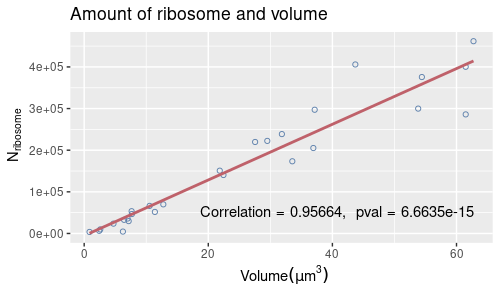
\includegraphics[width=0.5\columnwidth]{Exp_9_FCS/Figures/NvsVol_motbud}}\hfill
\subfloat[Density vs Volume\label{vdd}]{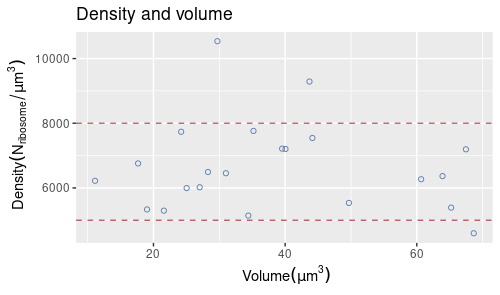
\includegraphics[width=0.5\columnwidth]{Exp_9_FCS/Figures/DvsV_wholecell}}
\caption{\textbf{A}: correlation plot of N$_{\text{ribosome}}$ against volume of individual mother and bud cells. 
\textbf{B}: plot of density against volume of whole cells (sum of mother + bud cells). 
Red dashed lines in \textbf{B} are only for illustrative purposes. }
\label{fig:corplot}
\end{figure}

The plot of N$_{\text{ribosome}}$ against the volume of each mother and bud cells (Fig.~\ref{nv}) demonstrates a positive, strong, and significant correlation (corr = 0.95). 
Which means that the N$_{\text{ribosome}}$ is not a constant value as previously believed, on the contrary, it is the density that is relatively constant (5000-8000 counts/$\mu$m$^3$).
This means that considering cells have different sizes, the number of ribosomes can not be used to indicate a cells state in the progression as demonstrated by the fact that a higher amount of N$_{\text{ribosome}}$ corresponds to larger cells (constant density). 
This is shown in Fig.~\ref{vdd} where the density varies rather constantly within the band as indicated by the (arbitrary) dashed line.

\begin{figure}[h!]
\centering
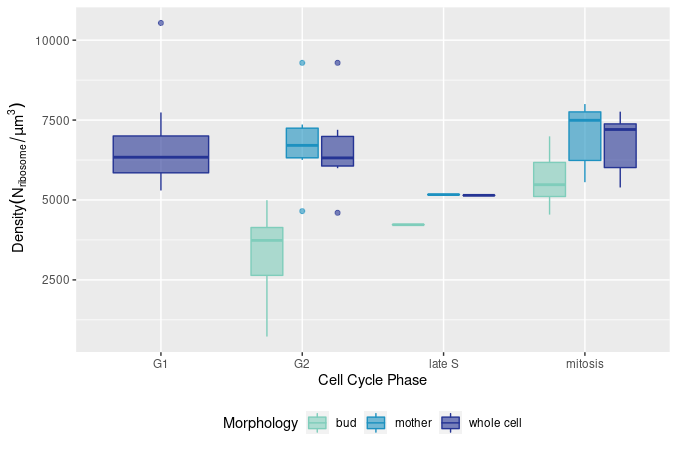
\includegraphics[width=0.9\columnwidth]{Exp_9_FCS/Figures/box_d_all}
\caption{Boxplot of density of different cell morphologies across the cell cycle. Whole cells in the G2, late S, and mitosis indicates the total density of mother and bud cells in these phases.}
\label{fig:bplot}
\end{figure}

The inability of this to distinguish cell morphology during cell cycle progression, or rather the constant value of density, is visualized by the boxplot in Fig.~\ref{fig:bplot} which shows that the density does not exhibit any meaningful change during the course of the cell cycle. 
The statistical test of which is supplied at the end of this chapter. In this case the late S phase is excluded from analysis due to insufficient amount of observation. 
The analysis by ANOVA for three cell cycle phases indicates no significant difference, hence not carried on further to test the individual differences by pairwise t-tests.

On the single cell level, however, discrimination between mother and bud cells is possible to be done with this technique by using the density as a measure. 
Separating the data shows that buds constantly exhibit a lower density in comparison to mother cells during the cycle from G2 up to mitosis (Fig.\ref{fig:bplot}). 
Evidence to this is further supported by statistical tests that found significant difference (by ANOVA for two groups: buds and mothers) between the density of buds and mother cells across the whole cell cycle progression (also supplied at the end of this chapter). 
Since only two groups was tested, no pairwise t-test was necessary.

Additional analysis was also done on the subset of buds. 
From the acquired data of this experiment, providing that singular observation is removed, it seems that even buds can be distinguished by the density according to which cell cycle phase they are currently in. 
The evidence is again supplied by the end of this chapter where ANOVA was carried on for two groups of cell cycle phase (G2 and mitosis) with result showing significant difference.



%----------------------------------------------------------------------------------------
%	BIBLIOGRAPHY
%----------------------------------------------------------------------------------------

\renewcommand{\refname}{\spacedlowsmallcaps{References}} % For modifying the bibliography heading
%\bibliographystyle{unsrt}

%\bibliography{sample.bib} % The file containing the bibliography
